\section{Équilibre électrostatique}
    Dans cette partie, nous allons appliquer la méthode de Newton-Raphson à l'électrostatique.
    Nous allons calculer la Jacobienne de $\nabla E$ pour pouvoir ensuite chercher les positions d'équilibre d'un système et enfin voir si ces solutions correspondent à un 
    maximum ou à un minimum de l'énergie.
\subsection{Jacobienne de $\nabla$$E(x_{1},x_{2},...,x_{N})$}
On considère qu'il existe N charges qui peuvent se déplacer dans l'intervalle [-1,1]. 
L'énergie électrostatique totale du système, E, se calcule avec la formule suivante.\\
\begin{equation*}
    E(x_{1},x_{2},...,x_{N})=\sum_{i=1}^{N}\left(ln|x_{i}+1|+ln|x_{i}-1|+\frac{1}{2}\sum_{j=1,j\not=i}^{N} ln|x_{i}-x_{j}|\right)
\end{equation*}
Les dérivées partielles de E peuvent se calculer ainsi :
\begin{equation*}
    \frac{\partial E(x_1, ..., x_N)}{\partial (x_i)} = \frac{1}{x_i+1} + \frac{1}{x_i-1} + \sum_{j=1,j\neq i}^{N} \frac{1}{x_i - x_j}
\end{equation*}
On a alors $\nabla E$ tel que : 
\begin{equation*}
    \nabla E(x_{1}, x_{2}, ..., x_{N}) = \left[\frac{\partial x_{i}}{\partial E(x_{1},...,x_{N})}\right]
\end{equation*}

On veut calculer la Jacobienne, J, de $\nabla E$. Pour ceci, on a implémenté les deux fonctions \verb|compute_jacob_diag_coeff| et \verb|compute_jacob_extra_coeff| qui calculent respectivement les coefficients diagonaux et les coefficients autres que ceux diagonaux de  la matrice Jacobienne de taille n² à l'aide des formules suivantes : 
\begin{equation*}
    J_{i,i} = \frac{\partial^2 E}{\partial x_i^2} = -\frac{1}{(x_i+1)^2} - \frac{1}{(x_i-1)^2} - \sum_{k=1, k\neq i}^{N} \frac{1}{(x_i - x_k)^2}
\end{equation*}
\begin{equation*}
    J_{i,j} = \frac{\partial^2 E}{\partial x_i \partial x_j} = -\frac{1}{(x_i - x_j)^2}
\end{equation*}

Après avoir implémenté ces deux fonctions, nous avons pu calculer la Jacobienne de $\nabla$E à l'aide de la fonction \verb|J_| qui utilise les deux fonctions précédentes. 
\subsection{Méthode de Newton-Raphson}
Ensuite, dans cette section, nous allons chercher les positions d'équilibre. Pour ce faire, nous allons résoudre à l'aide de la méthode de Newton-Raphson, l'équation suivante :
\begin{equation*}
    \nabla E(x_{1}, x_{2}, ..., x_{N}) = \left[\frac{\partial x_{i}}{\partial E(x_{1},...,x_{N})}\right]=0
\end{equation*}
Nous avons pris pour X le tableau : [-0.8,-0.5,0.1,0.5]. Nous avons donc appliqué à ce tableau, la fonction \verb|newton_raphson_backtracking| implémentée dans la Partie \ref{sec1}.
Nous avons ainsi obtenu comme racines : [-0.92954991, -0.82677351, -0.58010903, -0.00758336] auxquelles nous avons rajouté les points -1 et 1. Afin de mieux visualiser les racines obtenues, nous 
avons décidé de placer les points sur un graphe, ce que l'on peut voir sur la Figure \ref{fig:p2-c-legendre}. Sur ce même graphe, nous avons tracé les courbes des 
polynômes de Legendre. 
\begin{figure}[htbp!]
    \centering
    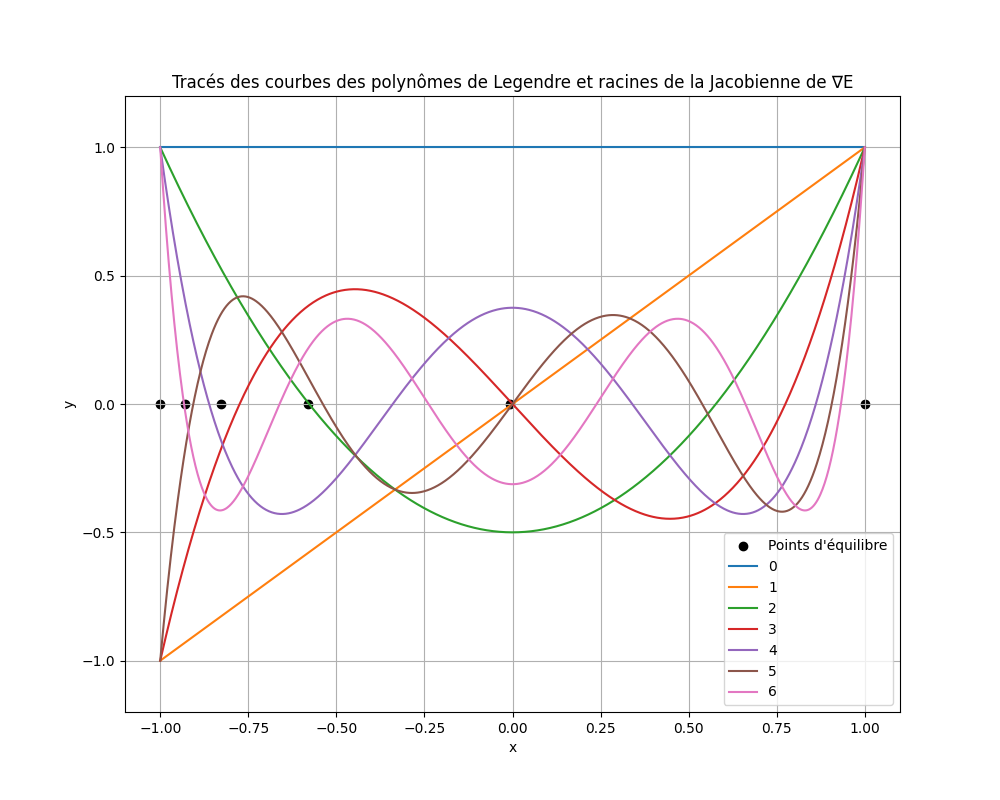
\includegraphics[width=0.65\textwidth]{res/part2_legendre.png}
    \caption{Représentation des courbes des polynômes de Legendre et des racines de la Jacobienne de $\nabla$E}
    \label{fig:p2-c-legendre}
\end{figure} 
On peut constater de manière graphique, sur la Figure \ref{fig:p2-c-legendre}, que la majorité des racines trouvées ressemblent
aux racines des dérivées des polynômes de Legendre. En effet, on peut voir qu'une des racines obtenues est proche de 0
tout comme l'est la racine des dérivées des polynômes de Legendre de degré impair, c'est-à-dire, de degré 1,3 et 5.
La racine proche de -0.58 est aussi proche de celle de la dérivée du polynôme de Legendre de degré 2.
Enfin, celle proche de -0.93 est proche de celle de la dérivée du polynôme de Legendre de degré 6.
\subsection{Maximum ou minimum de l'énergie électrostatique}
Enfin, nous avons cherché à savoir si les solutions correspondent à un maximum ou à un minimum de l'énergie électrostatique.
Pour cela, nous avons tracé l'énergie électrostatique en fonction de la position de la particule, x, ce que l'on peut 
voir sur la Figure \ref{fig:p2-c-2}. En effet, nous avons calculé E(x) pour des x allant de -1 à 1. 
\begin{figure}[htbp!]
    \centering
    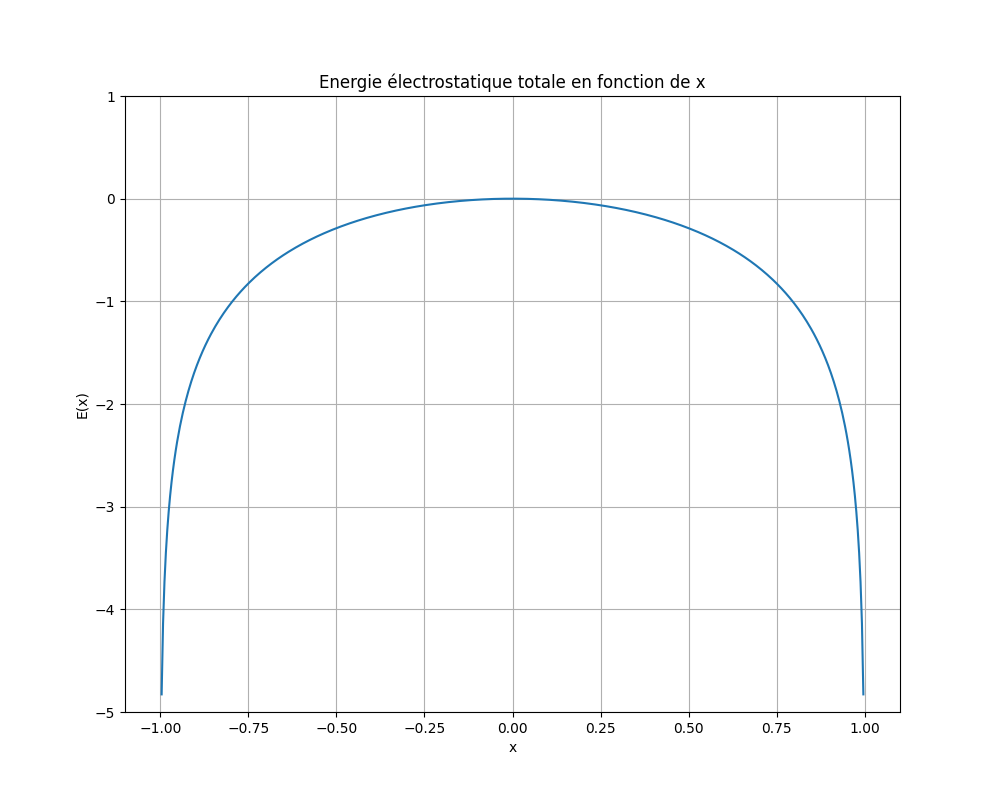
\includegraphics[width=0.65\textwidth]{res/part2_max_min.png}
    \caption{Graphe de l'Energie électrostatique totale en fonction de x}
    \label{fig:p2-c-2}
\end{figure} 
On peut voir sur la Figure \ref{fig:p2-c-2} que les solutions correspondent à un maximum de l'énergie électrostatique. 
En effet, le maximum est atteint en 0 sur le graphe.